% !TEX TS-program = pdflatex
% !TEX encoding = UTF-8 Unicode

% This is a simple template for a LaTeX document using the "article" class.
% See "book", "report", "letter" for other types of document.

\documentclass[11pt]{article} % use larger type; default would be 10pt

\usepackage[utf8]{inputenc} % set input encoding (not needed with XeLaTeX)

%%% Examples of Article customizations
% These packages are optional, depending whether you want the features they provide.
% See the LaTeX Companion or other references for full information.

%%% PAGE DIMENSIONS
\usepackage{geometry} % to change the page dimensions
\geometry{a4paper} % or letterpaper (US) or a5paper or....
% \geometry{margin=2in} % for example, change the margins to 2 inches all round
% \geometry{landscape} % set up the page for landscape
%   read geometry.pdf for detailed page layout information

\usepackage{graphicx} % support the \includegraphics command and options

% \usepackage[parfill]{parskip} % Activate to begin paragraphs with an empty line rather than an indent

%%% PACKAGES
\usepackage{booktabs} % for much better looking tables
\usepackage{array} % for better arrays (eg matrices) in maths
\usepackage{paralist} % very flexible & customisable lists (eg. enumerate/itemize, etc.)
\usepackage{verbatim} % adds environment for commenting out blocks of text & for better verbatim
\usepackage{subfig} % make it possible to include more than one captioned figure/table in a single float
% These packages are all incorporated in the memoir class to one degree or another...

\usepackage{hyperref}
\usepackage{amsmath, amssymb, amsthm}
\newtheorem{theoreme}{Theoreme}[section]
\newtheorem{definition}{Définition}[section]
\newtheorem{proposition}{Proposition}[section]
\newtheorem{corollary}{Corollary}[section]
\newtheorem{conjecture}{Conjecture}[section]
\usepackage{bbm}
%%% HEADERS & FOOTERS
\usepackage{fancyhdr} % This should be set AFTER setting up the page geometry
\pagestyle{fancy} % options: empty , plain , fancy
\renewcommand{\headrulewidth}{0pt} % customise the layout...
\lhead{}\chead{}\rhead{}
\lfoot{}\cfoot{\thepage}\rfoot{}

%%% SECTION TITLE APPEARANCE
\usepackage{sectsty}
\allsectionsfont{\sffamily\mdseries\upshape} % (See the fntguide.pdf for font help)
% (This matches ConTeXt defaults)

%%% ToC (table of contents) APPEARANCE
\usepackage[nottoc,notlof,notlot]{tocbibind} % Put the bibliography in the ToC
\usepackage[titles,subfigure]{tocloft} % Alter the style of the Table of Contents
\renewcommand{\cftsecfont}{\rmfamily\mdseries\upshape}
\renewcommand{\cftsecpagefont}{\rmfamily\mdseries\upshape} % No bold!

%%% END Article customizations

%%% The "real" document content comes below...

\title{Note modèles fractaux anisotropes}
\author{Leo Davy}
%\date{} % Activate to display a given date or no date (if empty),
         % otherwise the current date is printed 

\begin{document}
\maketitle
\section{Modèles isotropes}
\subsection{Mouvement brownien}
\begin{definition}
	On appelle mouvement brownien (en dimension $d$), tout processus mesurable $(B_t)_{t\in\mathbb{R}_+}$ à valeurs dans $\mathbb{R}^d$ vérifiant :
	\begin{enumerate}
		\item $B_0 = 0$ p.s.
		\item Le processus est à accroissements independants\footnote{Pour tout $t_1\leq t_2 \leq t_3$, on a que $B_{t_2} - B_{t_1}$ est indépendant de $B_{t_3} - B_{t_2}$.}
		\item $\forall s \leq t$ les accroissements suivent une loi normale $B_t - B_s \sim \mathcal{N}(0, (t-s)I_d)$\footnote{Implique stationarité ($\mu = 0$) du brownien, et isotropie ($\Sigma = \sigma I_d$)}
		\item Le processus est à trajectoire p.s. continues
	\end{enumerate}
\end{definition}
\begin{proposition}
	Soit $(B_t)$ un mouvement brownien
	\begin{enumerate}
		\item Pour tout $s>0$, on a que $B_t^s = B_{s+t} - B_s$ est un mouvement brownien\footnote{Indépendant de $\mathcal{F}_s = \sigma(\{B_u : u\leq s\})$}
		\item Pour tout $c>0$, $\tilde B_t = cB_{\frac{t}{c^2}}$ est un mouvement brownien
		\item On peut construire une isométrie\footnote{C'est à dire, que pour n'importe quel $f\in L^2(\mathbb{R}_+)$, on a que $\mathcal{W}(f)$ est une gaussienne centrée de variance $||f||_{L^2}$ et on a aussi $\mathbb{E}[\mathcal{W}(f_i)\mathcal{W}(f_j)] = \langle f_i, f_j\rangle_{L^2}$} entre les fonctions de carré intégrables classique $L^2(\mathbb{R}_+)$ (avec la mesure de Lebesgue), et $L^2(\Omega, \mathcal{F}, \mathbb{P})$ un espace de Gaussiennes indépendantes qui vérifie $\mathcal{W}(\mathbbm{1}_{[0,t]}) = B_t$...
	\end{enumerate}
\end{proposition}

\begin{theoreme}
	Une fonction $f:\mathbb{R}^d\to \mathbb{R}$ est définie positive si et seulement si il existe une mesure de probabilité symétrique $\mu$ sur $\mathbb{R}^d$ telle que 
	\begin{equation}
		\forall x \in \mathbb{R}^d,\quad f(x) = f(0)\int_{\mathbb{R}^d} e^{i\langle x, \xi \rangle} \mu(d\xi).
	\end{equation}
	C'est à dire qu'il existe un vecteur aléatoire symétrique $Z$ sur $\mathbb{R}^d$ tel que 
	\begin{equation}
				\forall x \in \mathbb{R}^d,\quad f(x) = f(0) \mathbb{E} e^{i\langle x, Z \rangle}.
	\end{equation}
\end{theoreme}
Conséquences du théorème (dans le cas où $(X_t)$ est un champ gaussien stationnaire)
\begin{proposition}
	\begin{enumerate}
		\item Si X est stationnaire et sa fonction d'autocovariance $K(t) = \mathbb{E}X_{s+t}X_s$ est continue, alors il existe une unique mesure finie $\mu$ sur $\mathbb{R}^d$ telle que 
			\begin{equation}
				K(t) = \int_{\mathbb{R}^d} e^{i\langle t, \xi\rangle}\mu(d\xi)
			\end{equation}
			appelée mesure spectrale du champ $X$.
		\item Si $K$ admet $\mu(d\xi) = f(\xi)d\xi$ comme densité spectrale, alors $f$ est définie positive et le champ gaussien $(Y_t)_t$ défini par
			\begin{equation}
				Y_t = \int_{\mathbb{R}^d} \sqrt{f(\xi)} e^{i\langle t, \xi\rangle} \hat{W}(d\xi)
			\end{equation}
			est indistinguable de $X$ et appelé représentation spectrale de $X$.
	\end{enumerate}
\end{proposition}
Dans le cas où le champ n'est pas nécessairement stationnaire mais a des accroissements stationnaires, on peut écrire la fonction de covariance par une mesure spectrale $\mu$ sous la forme
	\begin{equation}
		K(s,t) = \int_{\mathbb{R}} \left(e^{i\langle t,\xi\rangle} -1\right)\left(e^{-i\langle s, \xi\rangle} - 1\right)\mu(d\xi) + t\Sigma s
	\end{equation}
pour une certaine matrice $\sigma$ symétrique définie positive.
\newline
Et la représentation spectrale de $X$ devient, avec $\mu(d\xi) = f(\xi)d\xi$
\begin{equation}
	Y_t = \int_{\mathbb{R}^d} \left(e^{i\langle t, \xi \rangle} - 1\right) \sqrt{f(\xi)} \hat{W}(d\xi) + \langle t, N\rangle
\end{equation}
où $N$ est un vecteur gaussien centré de covariance $\Sigma$.
\subsection{Mouvement brownien fractionnaire}
Une première généralisation du mouvement brownien se fait par le mouvement brownien fractionnaire, en oubliant la condition d'avoir des accroissements indépendants.
\begin{definition}
	Soit $0<H<1$. Il existe un unique processus gaussien qui est $H$-autosimilaire, à accroissements stationnaires et tel que $Var(B_H(1)) = 1$. Le mouvement brownien fractionnaire $(B^H(t))_t$ est un tel processus, dont la covariance est donnée par 
	\begin{equation}
		Cov(B^H(t), B^H(s)) = \frac{t^{2H} + s^{2H} - |t-s|^{2H} }{2}
	\end{equation}
\end{definition}
$H$ est le coefficient de Hurst (que l'on considérera comme paramètre de régularité). 
\begin{itemize}
	\item	Si $H=\frac{1}{2}$, la corrélation est nulle, donc (par gaussianité) les accroissements sont indépendants et on retrouve le mouvement brownien.
	\item Si $H>\frac{1}{2}$, la corrélation est positive, donc les accroissements tendent  à avoir le même signe (le processus est dit persistant) et va donc avoir une forme de régularité.
	\item Si $H<\frac{1}{2}$, la corrélation est négative, les accroissements tendent à avoir des signes opposés et donc on aura beaucoup d'irrégularités.
\end{itemize}
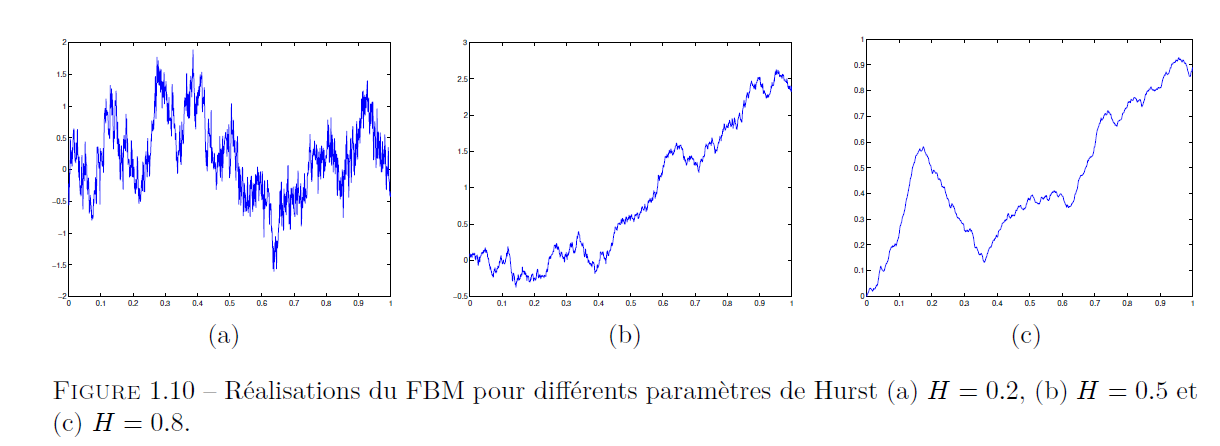
\includegraphics[width=1.2\textwidth]{hurst}
Deux représentations intégrales du mouvement brownien fractionnaire existent
\begin{proposition}
	\begin{enumerate}
		\item Par moyenne mobile
			\begin{equation}
				B^H(t) = \frac{1}{C_1(H)} \int_{\mathbb{R}} \left(  (t-x)_+^{H-\frac{1}{2}} - (-x)_+^{H - \frac{1}{2}} \right)
			\end{equation}
		\item Harmonisable
			\begin{equation}
				B^H(t) = \frac{1}{C_2(H)} \int_\mathbb{R} \frac{e^{it\xi} - 1}{|\xi|^{H+\frac{1}{2}}} \hat{W}(\xi)
			\end{equation}
	\end{enumerate}
\end{proposition}
Référence : Thèse Kévin Polisano, Chapitre 1
\section{Modèles anisotropes}
\subsection{Drap brownien fractionnaire}
Le premier modèle anisotrope est celui du drap brownien fractionnaire (Fractional Brownian Sheet - FBS). Dans celui-ci, on impose deux régularités $H_1$ et $H_2$ suivant chacun des axes. Moralement, c'est un produit de mouvements browniens fractionnaires.
\begin{definition}
	Le FBS $B^{H_1, H_2}$ est un champ gaussien centré, nul sur les axes, et de covariance
	\begin{align*}
		&\mathbb{E}\left[ B^{H_1, H_2}(x_1, x_2)B^{H_1, H_2}(x'_1, x'_2)\right]\\
			&= \frac{C_1(H_1)^2}{2} \left( |x_1|^{2H_1} + |x'_1|^{2H_1} -|x_1 - x'_1|^{2H_1}\right) \frac{C_1(H_2)^2}{2} \left( |x_2|^{2H_2} + |x'_2|^{2H_2} -|x_2 - x'_2|^{2H_2}\right) .
	\end{align*}
\end{definition}
\begin{proposition}
	Le FBS peut s'écrire sous les formes intégrales suivantes :
	\begin{enumerate}
		\item par moyenne mobile\footnote{Je crois que la variable d'intégration est $u,v$ plutôt que $x_1, x_2$}
			\begin{equation}
				B^{H_1, H_2}(x_1, x_2) = \frac{1}{C_1(H_1)C_1(H_2))}\int_{\mathbb{R}^2} f_{H_1}(x_1,u)f_{H_2}(x_2,v)dB(x_1, x_2)
			\end{equation}
			où $f_H(x,w) = (x - w)_+^{H - \frac{1}{2}} - (-x)_+^{H-\frac{1}{2}}$
		\item harmonisable
			\begin{equation}
				B^{H_1, H_2}(x_1, x_2) = \int_{\mathbb{R}^2} \frac{ (e^{ix_1\xi_1} - 1)(e^{ix_2\xi_2} - 1)}{|\xi_1|^{H_1 + \frac{1}{2}}|\xi_2|^{H_2 + \frac{1}{2}}}\hat{W}(\xi_1, \xi_2)
			\end{equation}
	\end{enumerate}
\end{proposition}

\subsection{Modèle de Bonami et Estrade}
	Un champ gaussien à accroissements stationnaires est caractérisé par son semi-variogramme
	\begin{equation}
		v_X(y) = \frac{1}{2}\mathbb{E}(X(y) - X(0))^2.
	\end{equation}
	En l'exprimant à partir de la mesure spectrale $\mu(d\xi) = f(\xi)d\xi$ associée à $X$, on peut alors réexprimer le champ sous la forme harmonisable
	\begin{equation}
		X^f(x) = \int_{\mathbb{R}^2} \left( e^{i\langle x, \xi\rangle} - 1\right) f(\xi)^{\frac{1}{2}}\hat{W}(d\xi).
	\end{equation}
	L'intérêt est qu'on peut alors caractériser les propriétés de symétrie de $X$ à partir de $f$.
	\begin{theoreme}
		\begin{enumerate}
			\item (Deux champs gaussiens stationnaires ont mêmes lois finies dimensionnelles si et seulement si ils ont le même variogramme)
			\item $X^f$ est autosimilaire si et seulement si $f$ est homogène
			\item $X^f$ est isotrope si et seulement si $f$ est radiale
		\end{enumerate}
	\end{theoreme}
	A partir de là, on peut construire des modèles avec des propriétés de régularité et d'autosimilarité en fixant $f$.
	\begin{enumerate}
		\item Fractional Brownian Field
		\begin{equation}
			\xi \mapsto \frac{1}{||\xi||^{2H + 2}}
		\end{equation} 
		\item Extended Fractional Brownian Field
		\begin{equation}
			\xi \mapsto \frac{1}{||\xi||^{2h(\xi) + 2}}
		\end{equation}
		où $\xi\mapsto h(\xi)$ est constante sur chaque direction et contrôle la régularité directionnelle.
		
		\item Operator Scaling Gaussian Random Field (hyperbolic wavelet transform)
		\begin{equation}
			f_{\theta_0, \alpha_0}(\xi) = |\zeta_1|^{1/\alpha_0} + |\zeta_2|^{1/(2-\alpha_0)}
		\end{equation}
		et on peut généraliser pour fixer au choix une propriété d'autosimilarité matricielle.
	\end{enumerate}
	Un modèle plutôt général de champ brownien anisotrope est donné par les champs browniens fractionnaires anisotropes définis par
	\begin{equation}
		f(\xi) = c(arg\xi)||\xi||^{-2h(arg(\xi)) - 2} 
	\end{equation}
	où $c$ et $h$ sont des fonctions $\pi$-périodiques qui permettent de controler les propriétés d'autosimilarité et d'anisotropie (en choisissant le degré d'homogénéité de $f$ via $h$ et l'anisotropie via $c$).
	\newline
	On a donc un modèle assez général de textures anisotropes spatialement homogène\footnote{La variation du champ dépend de la direction dans laquelle on regarde la variation, mais pas de la position d'où l'on regarde}, si maintenant on veut des modèles localement anisotropes , Polisano propose le modèle de champ brownien fractionnaire anisotrope généralisé.

	\begin{definition}
		Soient $h:\mathbb{R}^2 \to [0,1]$ et $C:\mathbb{R}^2\times\mathbb{R}^2 \to\mathbb{R}_+$ satisfaisant les hypothèses $\mathcal{H}$, on définit alors le champ brownien fractionnaire anisotrope généralisé par
	\begin{equation}
		X(x) = \int_{\mathbb{R}^2} (e^{i\langle x, \xi\rangle} - 1) \frac{C(x,\xi)}{||\xi||^{h(x) + 1}} \hat{W}(d\xi)
	\end{equation}

	\end{definition}
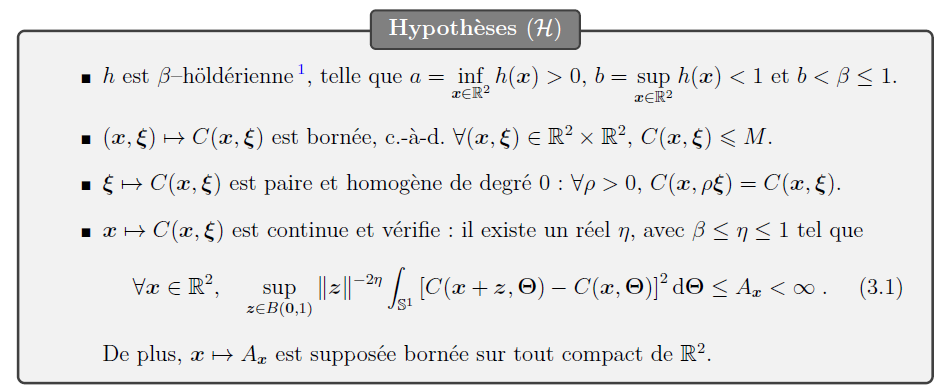
\includegraphics[width=1.\textwidth]{hypH}
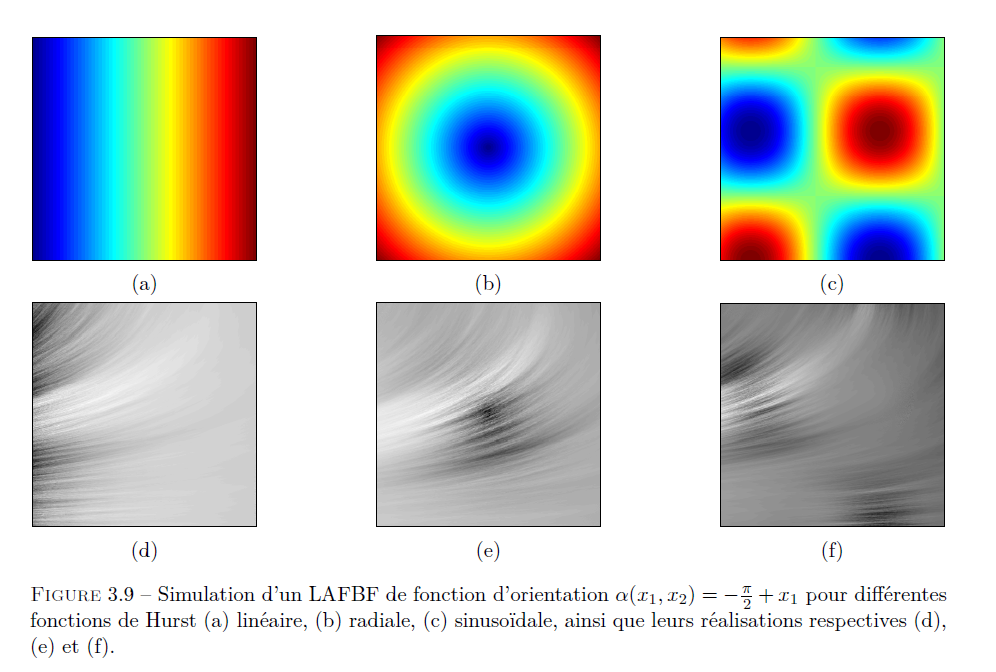
\includegraphics[width=1.\textwidth]{hurst_aniso}
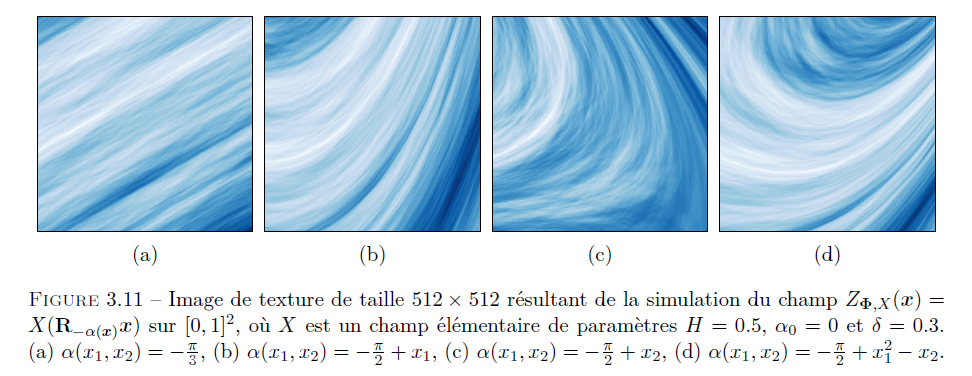
\includegraphics[width=1.\textwidth]{deform_elem}

\end{document}
